\section{Unit-Testing: An Overview}

At the first level of the code quality assurance process is the practice of ``unit-testing''. This process is a central tenet of test-driven software development and is widely established as a means of ``best-practice''. Before looking closely at the OpenQuake approach to unit-testing it is important to establish what are the precise objective of the unit-testing process and the benefits (and limitations) that it brings.

\subsubsection{Correctness of Implementation}

This objective is obviously the primary goal of unit-testing, to ensure that each function of the code is operating in the manner expected by the developer. ``Correctness'', in this case, requires that the function produces both the correct output, but also if there are cases in which function may fail then the means of failure should be predictable. The following is a relatively simple example of how a unit-test relates to a function:

Consider a simple function to multiply two numbers and take the logarithm of the result. A relevant analogy may be that of a magnitude scaling relation calculation, in which both a rupture length and rupture width are required, and the logarithm of the area may be needed by the function itself. In this circumstance a negative value in either of the two inputs would result in a calculation error. This could be coded in the following manner. 

\begin{lstlisting}[frame=single]
def get_log_area(length, width):
    if (length < 0) or (width < 0):
        raise valueError("Both inputs must be positive")
    else:
        return log10(length * width)
\end{lstlisting}

From the description above it is evident that the user requirements inform the manner in which the function should behave (i.e. negative values cannot be tolerated). To ensure that the function is operating correctly, we wish to write a set of tests that will confirm the behaviour is correct:

\begin{enumerate}
\item 1. If both $a$ and $b$ are equal to 10.0, then the function should return 2.0

\item If $a = -1$ and $b = 10$ the function should raise an error reporting the stated message ``Both inputs must be positive''.

\item If $a = 10$ and $b = -1$ the function should raise an error reporting the stated message ``Both inputs must be positive''.

\item If $a = -1$ and $b = -1$ the function should raise an error reporting the stated message ``Both inputs must be positive''.
\end{enumerate}

A unit-test for this function is an additional function that will check that both cases are satisfied, and will report an error if not. 

A comprehensive unit-test suite for a software may fulfil two objectives: \textbf{line coverage} and \textbf{parameter coverage}. The former should ensure that, in as far as possible, every line (or statement) in the code is executed as some point in the testing process. The latter should ensure that the behaviour of the function is predictable when supplied with ``unusual'' parameters. In the above example, both objectives are satisfied by the tests. The first test will result in a positive valued ``area'', thus executing the second branch of the logical path, the second test will result in a negative area and will execute the first logical branch. Therefore all lines of the code are covered and the line coverage is complete. We also see that in this simple example there are four possible cases: i) a is positive and b is positive, ii) a is positive and b is negative,  ii) a is negative and b is positive, and iv) both a and b are negative. Only the first case is valid, therefore the first test ensures that they provide the correct answer (usually verified by independent means), whilst the remaining tests should ensure that the function raises the correct error. Thus the full parameter space of the input is ensured.

The above case is, of course, trivial; however, as shall be seen in due course, this same process can be applied in more complex contexts. Furthermore, the same unit-testing approach can be applied not only to individual components within the PSHA calculation, but also to full calculations, essentially verifying that the hazard curve produced by the full PSHA calculator is in agreement with that produced independently (sometimes by hand).

\subsubsection{Identifies Problems Prior to Software Release}

This advantage is largely self-explanatory, but for many software projects this can reduce the possibility of requiring \emph{a posteriori} fixes to the code (patches). By compiling a comprehensive suite of unit-tests, and following a software development and release process that should automatically run the tests at the point of packaging, this should ensure that new features added to the software cannot inadvertently break other components.

\subsubsection{Facilities Improvements in Performance}

In the creation of software intended to perform demanding scientific calculations, like those commonly associated with PSHA, the issue of computational performance and efficiency is a major one. There is a continuing need to improve the speed and reduce the work required to undertake the PSHA calculation. To implement improvements it is necessary to ensure that optimisations do not modify the outputs of the calculation, only the speed at which they are performed. The unit-testing is absolutely fundamental to this process as optimisation cannot be undertaken readily without a means to ensure the calculation outputs have not changed. This point was a critical motivation behind the transition from the OpenSHA basis of the OpenQuake hazard calculation engine prior to version 1.0, to the current OpenQuake hazard library.

\section{Continuous Integration}

OpenQuake is developed and packaged within a ``continuous integration'' system (\href{https://ci.openquake.org/}{https://ci.openquake.org/}), which used the open-source software ``Jenkins'' (\href{http://jenkins-ci.org/}{http://jenkins-ci.org/}). Continuous integration is used in large software projects to run a full test suite of the complete software, either at fixed time intervals or, as in the current case, when any new code is committed to the repository. The continuous integration system will do the following:

\begin{enumerate}
\item Run the full set of unit-tests for all code in all of the linked repositories. This will include the main (or ``master'') branch of the software repository, i.e. the one that will be used for packaging of the software, as well as some development branches.

\item Run a test of the software installation. This test will install the software on a dedicated platform and check that the installation of the software is successful. This test also ensures that if changes occur in the dependency packages, and these changes affect or compromise the installation and operation of the software, these problems are recognised immediately.

\item The software will also run standard Python tests for quality of code, compilation of documentation etc.

\item Several long-running tests may also be run. These implement larger scale seismic hazard and risk calculations designed to test the overall performance of the engine. 
\end{enumerate}

If at any point the tests should fail, the OpenQuake development team will be notified automatically. This should ensure that software that is failing any of the tests will remain on the main branch of the repository for the minimum amount of time possible. Furthermore, if the continuous integration tests fail, the new code will not be integrated into the nightly package of the software. 

\section{The OpenQuake Hazard Library: Unit Tests}

The unit-test suite for the OpenQuake hazard library consists of three types of tests: i) simple tests for individual functions to verify the correctness of implementation (``component testing''), ii) simple tests of the full calculators for PSHA (``method testing''), and iii) ``acceptance'' tests, which provide a basic quality assurance check for the each of the three main calculators. 

\subsection{Component Testing}

The unit-testing at the component level breaks the functions into simple calculations whose results can be verified by hand. These tests, similar in nature to that illustrated previously, provide the majority of the line and parameter coverage needed to ensure a robust code. To illustrate the comprehensive nature of the coverage we consider the example of the functions to undertake calculations of geodetic distance between two points, which can be found here: \href{https://github.com/gem/oq-hazardlib/blob/master/openquake/hazardlib/geo/geodetic.py}{https://github.com/gem/oq-hazardlib/blob/master/openquake/hazardlib/geo/geodetic.py}. Whilst not necessarily a complex function in itself, the distance between two points on the Earth's surface is a critical component of the software that is frequently called at several points of the PSHA process. Therefore, it is critical that the function operates correctly and its behaviour under extreme cases is understood. Thus, this relatively simple function is verified in the following cases:

\begin{itemize}
\item \verb=test_LAX_to_JFK= Checks that a correct geodetic distance is calculated for two known locations on the Earth. This value is verified against an implementation of the algorithm provided by an online geodetic calculation tool.
\item \verb=test_on_equator= Checks that the correct distance is provided for two points located on the equator.
\item \verb=test_along_meridian= Checks that the correct distance is returned for two points located along the same meridian.
\item \verb=test_one_point_on_pole= Verifies the distance calculations for two points assuming one point is located at the geographic pole.
\item \verb=test_small_distance= Verifies that two points separated by a distance within the floating point error are considered to be separated by zero km
\item \verb=test_opposite_points= Verifies the correct distance between two points in different longitudinal hemispheres (i.e. checks that the distance crosses the international dateline correctly).
\item \verb=test_array= Verifies the correct distances between two set of points
\item \verb=test_one_to_many= Verifies the correct distances between one point and a set of points.
\end{itemize}

The test suite for this one function is illustrative of several key components of the unit-testing. First is the use of an independent tool to provide the expected values of the calculation under simple conditions. Second is the use of ``extreme cases'' such as polar locations, or across the International Dateline. These ensure that the function can be global in application. 

The nature of the interdependencies between the functions also means that one a functions own unit-test is verified, the function can then form the basis for testing other conditions. So for example, the geodetic distance tools also contain a method to calculate the minimum distance between a collection of points and a single point. Rather than requiring new expected distances for the different conditions, the geodetic distance function can then be used to construct tests for functions that utilise it. This makes the testing process more efficient, and reduced the need to write large numbers of tests in order to ensure correct behaviour of the function.

\subsection{Ground Motion Prediction Equation (GMPE) Testing}

The implementation process for ground motion prediction equations requires careful consideration, as it is in this area that new features may be expected to be added regularly, and where contributions from third parties are more likely to be incorporated into the software. Furthermore, in most cases the expected values of the functions may only be obtained from independent implementations of the GMPE. These expected values take the form of test tables, which are simple comma-separated value (csv) files that provide the expected values and standard deviations of the ground motion prediction equation for an exhaustive combination of parameters for the predictor variables. These should be sufficient to ensure that every part of the GMPE is covered within the test. An example test table is shown in Figure \ref{fig:gmpe_test_table}.

\begin{figure}[htbp]
  \centering
  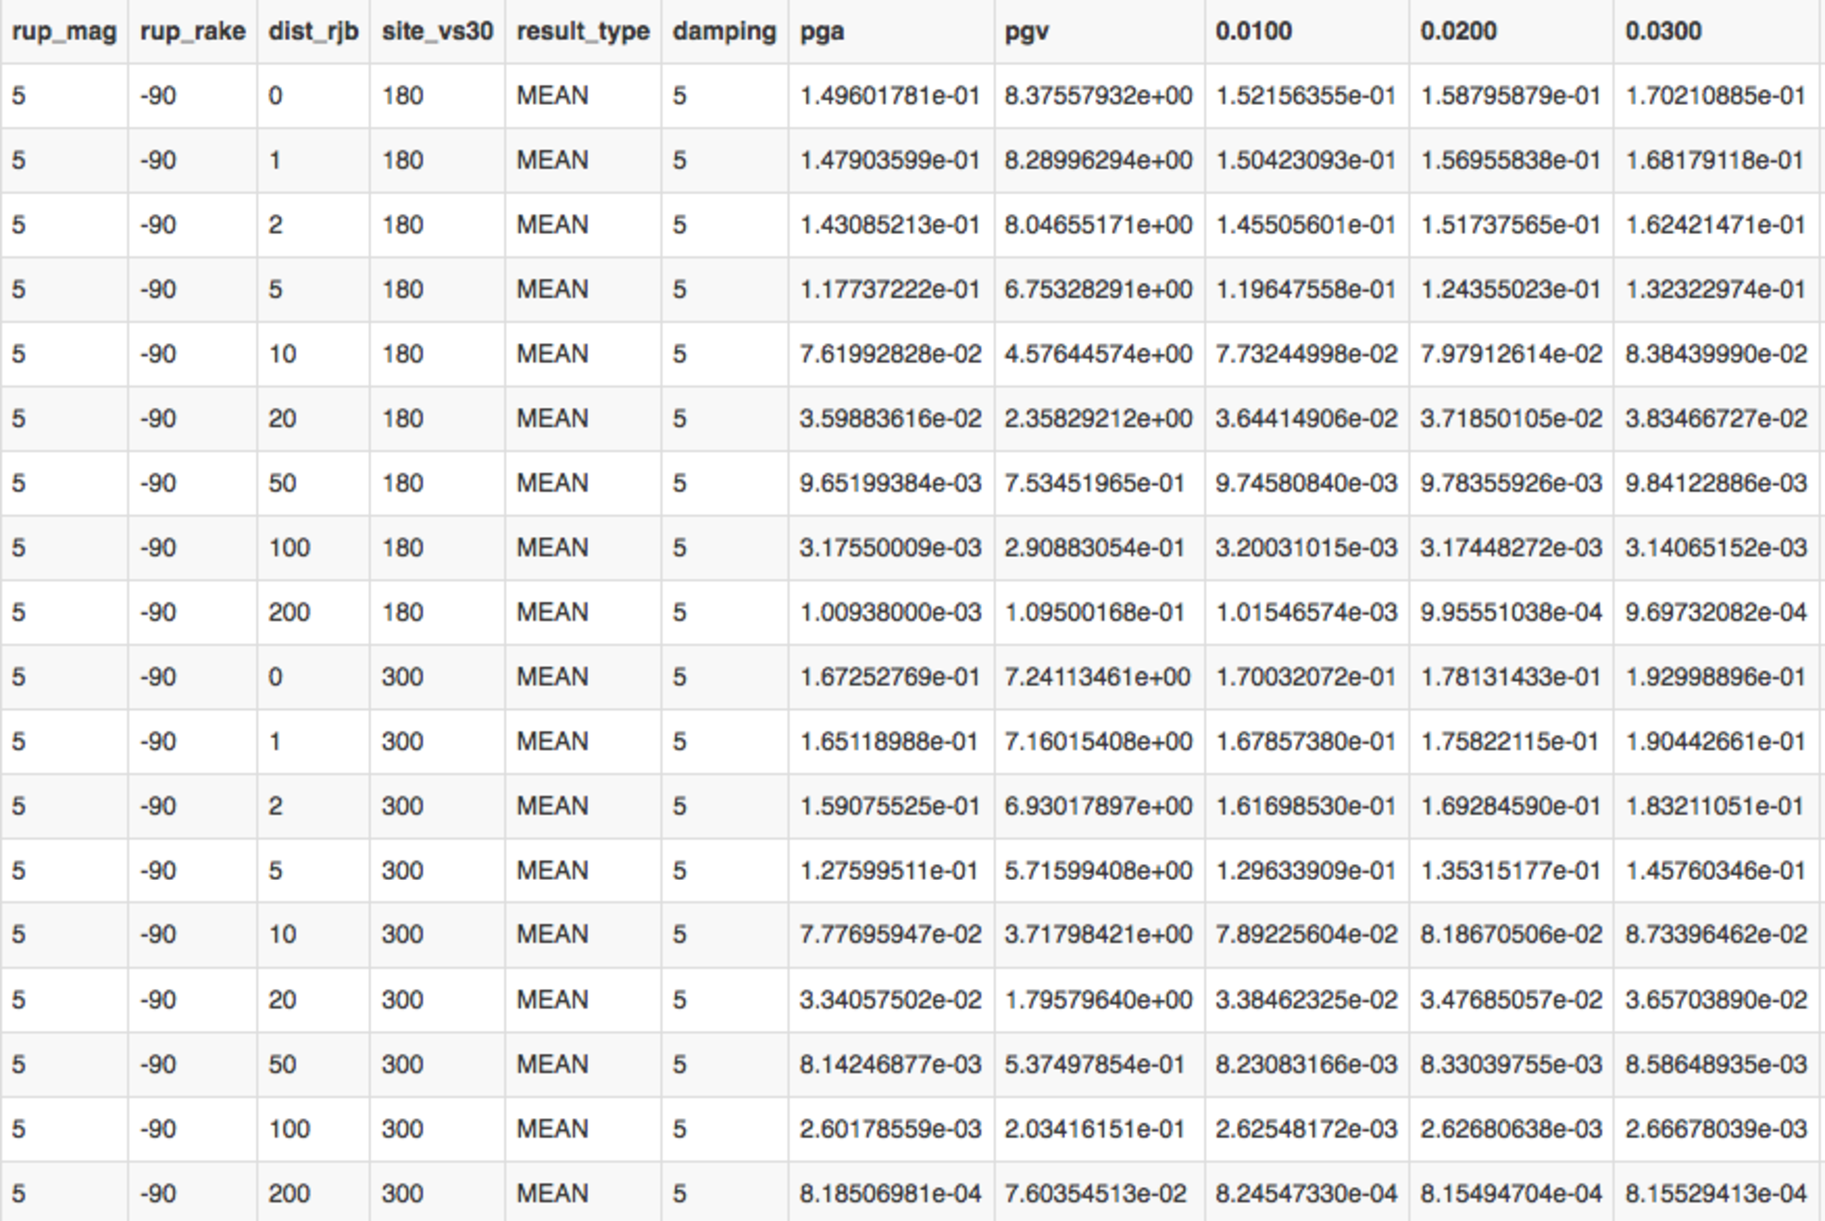
\includegraphics[width=0.8\textwidth]{./qareport/pictures/test_tables_screen_capture.pdf}
  \caption{Example GMPE test table used by OpenQuake}
  \label{fig:gmpe_test_table}
\end{figure}

To ensure the most objective testing strategy, we aim for the test tables to match the GMPE creator's own implementation of the GMPE, in as far as possible. Therefore we prefer to solicit input from the authors of the GMPE. This will often take one of two forms. We ask that the authors can provide test tables, in a convenient format, or that they provide their own software implementation of the GMPE, from which we will then generate the test tables. Input from the GMPE authors is highly desirable within this process as it can help resolve issues that are perhaps ambiguous within the original publications of the GMPE and it can identify errors and bugs in the author's own implementation. The full workflow for GMPE implementation in OpenQuake is shown in Figure \ref{fig:gmpe_flowchart}.

\begin{figure}[htbp]
  \centering
  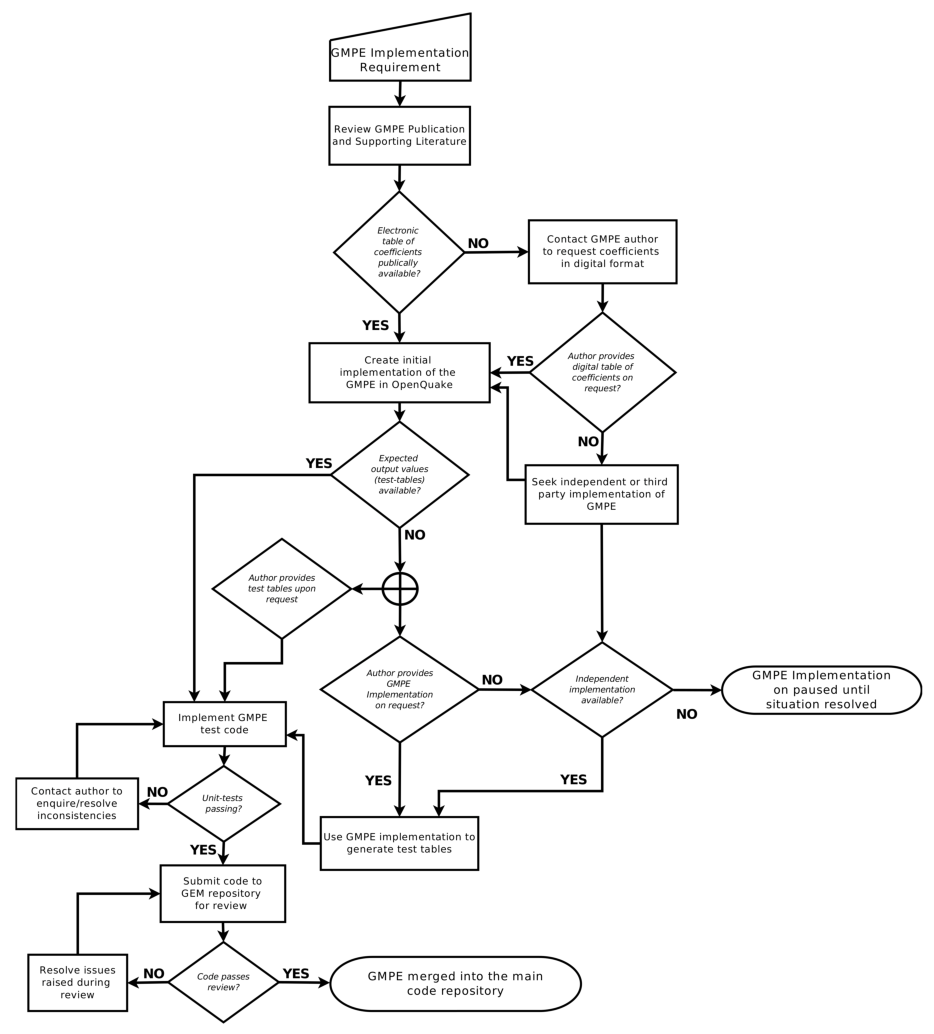
\includegraphics[width=\textwidth]{./qareport/pictures/gmpe_implementation_flowchart.pdf}
  \caption{OpenQuake GMPE Implementation Process}
  \label{fig:gmpe_flowchart}
\end{figure}

The GMPE unit-tests themselves are designed to be simple for the user to create once the test tables are provided. Ideally the expected values should match the implementation values to within the test precision (typically permitting a difference of $10^{-7}$). In some cases, however, it may not be possible to match the desired level of precision and therefore the tests permit the maximum discrepancy level (as a percentage) to be specified. Discrepancies may arise due to rounding of the coefficients within published tables, but ideally the tolerable discrepancy between an expected and predicted value should be not more than one tenth of one percent.

As is shown from Figure \ref{fig:gmpe_flowchart}, once the GMPE test tables are created, the GMPE implementation should then be checked against the unit-tests. If discrepancies cannot obviously be resolved the author may then be contacted for clarification. Once the unit-tests pass the code is then submitted for review by (typically) one or more of the software development team and one or more of the scientific team. This may help identify issues such as inefficiencies or unclear code. Once the submission is accepted by both the scientific and IT reviewer the code is merged into the main repository. This will then trigger a full test from the continuous integration system described previously.


\section{Acceptance Tests}

In addition to the individual unit-tests on functions, the OpenQuake hazard library contains three code ``acceptance'' tests. These are tests that are designed to exercise the full workflow of the classical, event-based and disaggregation calculators. Further comprehensive tests of all of the main OpenQuake calculators are also found in the test suite of the main OpenQuake engine, and these shall be elaborated upon in section ??.

\subsection{Classical PSHA Acceptance Tests}

The following tests, taken from the PEER tests suite \citep{thomas2010}, are used as the the basis for the unit tests of the classical PSHA calculation engine:

\begin{enumerate}
\item \textbf{Set 1 Case 10} 

This test considers one uniform area source with a truncated exponential model with $M_{min}$ of 5.0, $M_{max}$ 6.5, b-value of 0.9 and an annual rate $M_W \geq M_{min}$ of 0.0395. As OpenQuake defines finite rupture planes for each of the points considered in the area source, the scaling relation was fixed such that the area of the finite rupture was equal to 1.0 km. Hypocentral depth is fixed at 5 km. The preferred GMPE is \cite{sEtAl1997} for rock, with sigma set to 0.0. The expected values for the unit tests are those provided in the appendix of \cite{thomas2010} (page A - 15), which represent the mean values of the distribution of estimates from the software considered. As these are not solved by hand, the test are considered to pass when the following condition is satisfied for all values:

\begin{equation}
|calculated - expected| \leq \left( {atol + rtol * |expected|} \right)
\end{equation}

where $atol$ and $rtol$ are the absolute and relative difference between two terms, set to $10^{-4}$ and $10^{-1}$ respectively.

\item \textbf{Set 1 Case 11}

The same area source and GMPE are considered as for \textbf{Set 1 Case 10}; however, the hypocentral depth is distributed uniformly between 5 km and 10 km. All other conditions are the same.


\item \textbf{Set 1 Case 2}

This case considered a vertical strike-slip planar fault rupture with a single magnitude $M_W$ 6.0, whose expected rupture plane is smaller than the total area of the fault. The slip rate is assumed to be $2 mm yr^{1}$, giving an annual recurrance of 0.0160425 $yr^{-1}$. The following scaling relations are used, which in combination give an expected aspect ratio equal to 2.0.

\begin{eqnarray}
\log_{10} A &=& M_W - 4.0\\
\log_{10} W &=& 0.5 M_W - 2.15\\
\log_{10} L &=& 0.5 M_W - 1.85
\end{eqnarray}

where $A$, $W$ and $L$ are the rupture area, width and length respectively. The GMPE, site condition and sigma truncation are the same as for \textbf{Set 1 Case 10} and \textbf{Set 1 Case 11}


\item \textbf{Set 1 Case 5}

This case considers the same fault plane as in \textbf{Set 1 Case 2} albeit with an exponential magnitude frequency distribution with $M_{MIN}$ and $M_{MAX}$ of 5.0 and 6.5 respectively and a b-value of 0.9. The same slip rate is assumed, which translates into an a-value of 3.1292. All other inputs are the same.
\end{enumerate}


\subsection{Event-Based PSHA Acceptance Tests}

The event-based acceptance tests are designed to verify that for a sufficiently long stochastically generated catalogue originating from an area source, $10^6$ years in this case, the normalised rate of events in each magnitude frequency bin is approximately equal to that of the expected magnitude frequency distribution. This is expanded to check out source to site distance filtering by considering a second source beyond the expected soure-to-site distance filter range. 

\subsection{Deaggregation Acceptance Tests}

The disaggregation calculator is tested in two separate places. A first unit-test evaluates the disaggregation of hazard for a simple case in which the probabilities in the disaggregations bins have been calculated, by hand, for a simple rupture model. This unit-test will fulfil the requirements of line and parameter coverage, including edge cases such as if the rupture crosses the international dateline, or if no ruptures contribute to the hazard at the site. A second unit-test using a more realistic source and GMPE combination are then implemented. In this case it is not possible to calculate the probabilities by hand, but instead the OpenQuake results are used as the expected values. This test is circular in nature, and is intended simply as a means to ensure that changes to the code do not alter the results of the disaggregation calculator.

\section{Summary}

In this section we have outlined both the process and the key benefits of developing comprehensive unit-tests for OpenQuake, as well as outlining the operation of the continuous integration system, which should ensure that code with the potential to break the tests cannot be packaged and released. The unit-tests themselves have not been discussed in detail as nearly one thousand tests are executed during the unit-test process. However, to view the comprehensive set of tests reader is encouraged to refer to the full test-suite, which is open and available on the OpenQuake code repository (\href{https://github.com/gem/oq-hazardlib/tree/master/openquake/hazardlib/tests}{https://github.com/gem/oq-hazardlib/tree/master/openquake/hazardlib/tests}). Furthermore, we have also discussed how OpenQuake development tries to facilitate correct implementation of features such as ground motion prediction equations. For relatively simple conditions, a selection of PEER tests \citep{thomas2010} are built into the testing process, making OpenQuake unique amongst other hazard software in integrating the verification into the development process. The following chapters will expand in greater detail upon the additional hazard curve benchmark tests, which both follow and expand upon the PEER testing process. T



